\documentclass{beamer}
\usepackage{listings}
\usepackage{graphicx}
%\usepackage{beamerthemesplit}
 \usetheme{Goettingen}

% \usetheme{default}
% \usetheme{Boadilla}
% \usetheme{Madrid}
% \usetheme{Montpellier}
% \usetheme{Warsaw}
% \usetheme{Copenhagen}
 \usetheme{Goettingen}
% \usetheme{Hannover}
% \usetheme{Berkeley}
 
% \usecolortheme{crane}
 % \beamertemplatesolidbackgroundcolor{craneorange!25}




\title{Python in Neurocomputation - A Brief Introduction}
\author{Mike Hull}
\date{\today}

\begin{document}

\frame{\titlepage}

\section[Outline]{}
\frame{\tableofcontents}









\section{Motivation}
\subsection{What?}
\frame
{
  \frametitle{What is Python?}

  \begin{itemize}
  \item<1-> High-level, general purpose programming language
  \item<2-> In development since 1989. Currently Version 2.6
  \item<3-> Opensource - Strong User Community  
  \item<4-> Used by \ldots
	  \begin{itemize}
		  \item Google - google-mail, google-groups \& google-maps
		  \item Yahoo! - discussion boards
	  \end{itemize}
  \item<5-> Popular as an interface to software: GIMP, Blender, Maya, SPSS, neuron
  \end{itemize}
}


\subsection{Why}
\frame
{
  \frametitle{Why is Python Popular?}

  \begin{itemize}
  \item<1-> Design Philosophy
	  \begin{itemize}
	  \item<2-> `remarkable power with very clear syntax'
	  \item<3-> `to describe something as clever is \emph{NOT} considered a compliment in the Python culture'
	  \end{itemize}
  \item<4-> Learning Curve
  \item<5-> Scalability
  \item<6-> Cross Platform
  \item<7-> Standard Library - databasing, cryptography, networking, graphics, \ldots
  \item<8-> Extensibility
  \item<9-> Rapid Development
  \item<10-> \ldots Programming Python is Fun!! 
  \end{itemize}
}


\makeatletter
\let \@sverbatim \@verbatim
\def \@verbatim {\@sverbatim \verbatimplus}
{\catcode`'=13 \gdef \verbatimplus{\catcode`'=13 \chardef '=13 }} 
\makeatother



\subsection{How?}
\begin{frame}[fragile]
  \frametitle{How does Python look?}

  \small

\begin{verbatim}
#Example 1
height = 12.5
weight = 23.8
area = height * weight
print area
>> 297.5
\end{verbatim}

\begin{verbatim}
#Example 2
a = 'Xenopus'
b = 'laevis'
print 'Lets study ' + a + ' ' + b + '.'
>> Lets study Xenopus laevis.
\end{verbatim}


\end{frame}



\section{A Brief Tour}
\subsection{Basic Data Types}

\subsection{Basic Data Types}
\begin{frame}[fragile]
  \frametitle{Basic Built-in Data Types}
  \begin{itemize}

    \item<1-> Integer
    \item<2-> Float
    \item<3-> String
  \end{itemize}

  \begin{itemize}
    \item<4-> Lists
    \item<5-> Dictionary
  \end{itemize}

  \begin{itemize}
    \item<6-> Tuples
    \item<7-> \begin{verbatim} None True False \end{verbatim}
  \end{itemize}

\end{frame}


\begin{frame}[fragile]
  \frametitle{Basic Data Types}



  \begin{itemize}
  \item<1-> Integer, Float
	  \begin{list}{\quad}{}
		  \small
		  \item<2-> \begin{verbatim} >>> (50-5*6)/4 \end{verbatim}	
		  \item<3-> \begin{verbatim} 5 \end{verbatim}	
		  \item<4-> \begin{verbatim} >>> 3 * 3.75 / 1.5 \end{verbatim}	
		  \item<5-> \begin{verbatim} 7.5 \end{verbatim}	
	  \end{list}

  \item<6-> String
	  \begin{list}{\quad}{}
		  \small
		  \item<7-> \begin{verbatim} >>> 'Hello, ' + 'plymouth' \end{verbatim}	
		  \item<8-> \begin{verbatim} 'Hello, plymouth' \end{verbatim}	
		  \item<9-> \begin{verbatim} >>> a = 'Bristol has hills'
 >>> a[0]	  \end{verbatim}	
		  \item<10-> \begin{verbatim} 'B' \end{verbatim}	
 		  \item<11-> \begin{verbatim} >>> a[1]	  \end{verbatim}	
		  \item<12-> \begin{verbatim} 'r' \end{verbatim}	
 		  \item<13-> \begin{verbatim} >>> len(a)	  \end{verbatim}	
		  \item<14-> \begin{verbatim} 18 \end{verbatim}	
	  \end{list}

  \end{itemize}
\end{frame}



\subsection{Lists \& Dictionaries}
\begin{frame}[fragile]
  
	\frametitle{Lists}

	  \begin{list}{\quad}{}
		  \small
		  \item<1-> \begin{verbatim} >>> l = [2,3,5,7,11,13] \end{verbatim}	
 		  \item<2-> \begin{verbatim} >>> l[0]	  \end{verbatim}	
		  \item<3-> \begin{verbatim} 2 \end{verbatim}	
 		  \item<4-> \begin{verbatim} >>> len(l)	  \end{verbatim}	
		  \item<5-> \begin{verbatim} 6 \end{verbatim}	
 		  \item<6-> \begin{verbatim} >>> for x in l:	  
 >>>     print 'Item: ', x, ', Doubled: ', x*2, \end{verbatim}	
		  \item<7-> \begin{verbatim} Item: 2, Doubled: 4
 Item: 3, Doubled: 6
 Item: 5, Doubled: 10
 Item: 7, Doubled: 14
 Item: 11, Doubled: 22
 Item: 13, Doubled: 26 \end{verbatim}	
		 \item<8-> \begin{verbatim} >>> l = ['neuron', 'axon', 'dendrite', 4.6, 16] \end{verbatim}	
	  \end{list}


\end{frame}







\begin{frame}[fragile]
  
  \frametitle{Dictionaries}

  \begin{itemize}
	  \item<1-> Dictionaries map a \emph{key} to a \emph{value}
	  \begin{list}{\quad}{}
		  \footnotesize
		  \item<2-> \begin{verbatim} >>> channel_density = { 
                   'soma':  1.0, 
                   'dendrite': 0.8,
                   'axon':0.7,
                   'axonhillock':  1.7,
                    }
				   
				   \end{verbatim}	
 		  
	\item<3-> \begin{verbatim} 
 >>> channel_density['axon']	  \end{verbatim}	
	\item<4-> \begin{verbatim} 0.7

		\end{verbatim}	
	\item<5-> \begin{verbatim} 
 >>> channel_density['axonhillock']	  \end{verbatim}	
	\item<6-> \begin{verbatim} 1.7	  \end{verbatim}	
	  \end{list}

  \end{itemize}
\end{frame}

\begin{frame}[fragile]
  
  \frametitle{Dictionary Iteration}

	  \begin{list}{\quad}{}
		  \tiny
		  \item<2-> \begin{verbatim} >>> regions = channel_density.keys() \end{verbatim}	
		  \item<3-> \begin{verbatim} >>> regions \end{verbatim}	
		  \item<4-> \begin{verbatim} >>> ['axon','dendrite','soma','axonhillock']  \end{verbatim}	

		  \item<5-> \begin{verbatim} >>> for location in residence.keys():
	        	print location + ' has channel density ',  channel_density[location]
			  \end{verbatim}

		  \item<6-> \begin{verbatim} 
		 axon has channel density 1.0
		 dendrite has channel density 0.8
		 soma has channel density 1.0
		 axonhillock has a channel density 1.7
		 \end{verbatim} 

	  \end{list}
 		  

\end{frame}



















\section{Example - Manipulating an SWC File}
\subsection{Background}
\begin{frame}[fragile]
 
  \frametitle{Example 1}

  \begin{itemize}
  \item<1-> Load SWC File and calculate the surface area of the neuron
  \item<2-> SWC File Format
	  \begin{list}{\quad}{}
		  \item<2-> ID TYPE XPOS, YPOS, ZPOS, RAD, PARENT\_ID
		  \item<3-> \begin{verbatim}
54	2	0.00	-3.00	-3.00	0.15	-1
55	51	0.50	-5.00	-4.00	0.50	54
56	51	0.00	-7.00	-7.00	0.15	55
\end{verbatim}
\end{list}
  \item<4-> Surface Area of cylinder: $A = (R+r) \times \pi \times length $
  \end{itemize}

\end{frame}


\subsection{Algorithms}
\begin{frame}[fragile]
 
  \frametitle{Human Algorithm}
  \begin{itemize}
	%\scriptsize
	  \item<1-> For each line in the file (without a parent\_id -1):
	  \begin{itemize}
	%\scriptsize
		  \item<2-> Find the position and radius of the parent.
		  \item<3-> Find the length of the segment by subtracting this lines position for the parents (via Pythagorus)
		  \item<4-> Calculate the surface area of this segment using length and radii
	  \end{itemize}
	  \item<5-> Add up the surface area of all lines. 
  \end{itemize}
	
\end{frame}

\begin{frame}[fragile]
 
  \frametitle{Python Algorithm}

  \begin{itemize}
	\footnotesize
		
	\item<1-> Read all the lines in the file \& create a dictionary with the data, 	  
	\begin{list}{\quad}{}
		  \item<2-> Map id's to a list containing the data on the line: $ id \mapsto [ x,y,z,r, parent\_id ] $
		  \item<3-> $ 54 \mapsto [0.00, -3.00, -3.00, 0.15, -1] $
		  \item<4-> $ 55 \mapsto [0.00, -5.00, -4.00, 0.50, 54] $
		  \item<5-> $ 56 \mapsto [0.00, -7.00, -7.00, 0.15, 55] $
	  \end{list}
  \item<6-> Iterate over every id in the dictionary (without a parent\_id of -1):
	\begin{list}{\quad}{}
		  \item<7-> Lookup the data($[x,y,z,r,parent\_id]$) for that id in the dictionary
		  \item<8-> Lookup the parent\_data using parent\_id (again using the dictionary)
		  \item<9-> Calculate the length of the segment
		  \item<10-> Calculate the surface of the segment
		  
	  \end{list}
	  \item<11-> Add up the surface area of all id's. 

  \end{itemize}

\end{frame}






\subsection{Implementation}
\begin{frame}[fragile]
	\frametitle{Reading the File I}
	\scriptsize

\begin{block}{Program}
\begin{verbatim}
swcFile = open( "myNeuron.swc")
for line in swcFile.readlines():
    print line,
\end{verbatim}
\end{block}

\begin{block}{Output}
\begin{verbatim}
'54	2	0.00	-3.00	-3.00	0.15	-1'
'55	51	0.50	-5.00	-4.00	0.50	54'
'56	51	0.00	-7.00	-7.00	0.15	55'
...
'77	2	8.00	-8.00	-27.00	0.15	76'
\end{verbatim}
\end{block}
\end{frame}




\begin{frame}[fragile]
	\frametitle{Reading the File II}
	\scriptsize

\begin{block}{Program}
\begin{verbatim}
swcFile = open( "myNeuron.swc")
for line in swcFile.readlines():
    lineSplit = line.split()
    print lineSplit
\end{verbatim}
\end{block}

\begin{block}{Output}
\begin{verbatim}
['54',	'2',	'0.00',	'-3.00',	'-3.00',	'0.15',	'-1']
['55',	'51',	'0.50',	'-5.00',	'-4.00',	'0.50',	'54']
['56',	'51',	'0.00',	'-7.00',	'-7.00',	'0.15',	'55']
...
['77',	'2',	'8.00',	'-8.00',	'-27.00',	'0.15',	'76']
\end{verbatim}
\end{block}
\end{frame}




\begin{frame}[fragile]
	\frametitle{Extracting the data}
	\scriptsize

\begin{block}{Program}
\begin{verbatim}
swcFile = open( "myNeuron.swc")
for line in swcFile.readlines():
    lineSplit = line.split()
	
    id = int( lineSplit[0] )
    x = float( lineSplit[2] ) 
    y = float( lineSplit[3] ) 
    z = float( lineSplit[4] ) 
    r = float( lineSplit[5] ) 
    parent_id = int( lineSplit[6] ) 

    print 'ID: %d (%f,%f,%f) R:%f Parent:%d' % (id,x,y,z,r,parent_id)
\end{verbatim}
\end{block}

\begin{block}{Output}

\begin{verbatim}
ID: 54 (0.00,-3.00,-3.00) R:0.15 Parent:-1]
ID: 55,(0.50,-5.00,-4.00) R:0.50 Parent:54]
ID: 56,(0.00,-7.00,-7.00) R:0.15 Parent:55]
...
ID: 77,(8.00,-8.00,-27.00) R:0.15 Parent:76]
\end{verbatim}
\end{block}
\end{frame}


\begin{frame}[fragile]
	\frametitle{Building the Dictionary}
	\scriptsize

\begin{block}{Program}
\begin{verbatim}
idDict = {}
swcFile = open( "myNeuron.swc")
for line in swcFile.readlines():
    lineSplit = line.split()
	
    id = int( lineSplit[0] )
    x = float( lineSplit[2] ) 
    y = float( lineSplit[3] ) 
    z = float( lineSplit[4] ) 
    r = float( lineSplit[5] ) 
    parent_id = int( lineSplit[6] ) 
	
    idDict[id] = [x,y,z,r,parent_id]

print idDict
\end{verbatim}
\end{block}

\begin{block}{Output}
\begin{verbatim} { 54 :[0.00,-3.00,-3.00,0.15,-1], 55:[0.50,-5.00,-4.00,0.50,54], 
56:[0.00,-7.00,-7.00,0.15,55], ... 77:[8.00,-8.00,-27.00,0.15,76] }
\end{verbatim}
\end{block}
\end{frame}





















\begin{frame}[fragile]
	\frametitle{Calculating the Surface Areas}
	\tiny

\begin{verbatim}
from math import pi,sqrt
def calcLength(x1,y1,z1, x2,y2,z2):
    x = x1-x2
    y = y1-y2
    z = z1-z2
    return sqrt( x*x + y*y + z*z )

total_area = 0
for id, swcData in idDict.iteritems():
    #Shorthand for:x = swcData[0], y = swcData[1] ...
    x,y,z,rad,parent_id = swcData

    if parent_id == -1:
        print "ID: %d - Root node - nothing to do" %id
    else:
        parent_swc_data = idDictionary[ parent_id ]
        p_x,p_y,p_z,p_rad,p_parent_id = parent_swc_data
    
        l = calcLength(x,y,z, p_x,p_y,p_z)
        sa = (rad + p_rad) * pi * l
        print "ID: %d - Length %f, SA: %f" % (id,l,sa)    
        total_area = total_area + sa
print 'Total Area:', total_area \end{verbatim}

\begin{verbatim}ID: 55 - Root node - nothing to do"
ID: 56 - Length 3.64, SA: 7.43                                                                   
ID: 57 - Length 1.50, SA: 3.06                                                                   
...
ID: 77 - Length 2.24, SA: 2.11
Total Area: 98.78
\end{verbatim}
%\end{block}
\end{frame}







\begin{frame}[fragile]
	\frametitle{Condensing}
	\tiny

\begin{block}{Simplfied Program}
\begin{verbatim}
from math import pi,sqrt
from numpy import array
from scipy.linalg import norm

swcFile = open("myNeuron.swc")
for line in swcFile.readlines():
    lineSplit = line.split()
    
    id = int( lineSplit[0] )
    xyz = array( [float(lineSplit[2]), float(lineSplit[3]), float(lineSplit[4]) ] )
    r = float( lineSplit[5] ) 
    parent_id = int( lineSplit[6] ) 
    idDict[id] = [xyz,r,parent_id]

segmentAreas = {}
for id, (xyz,rad,parent_id) in idDict.iteritems():
    if parent_id == -1: continue
        
    p_xyz,p_rad,p_parent_id = idDictionary[ parent_id ]
    segmentAreas[id] = (rad + p_rad) * pi * norm(p_xyz-xyz)

print 'Total Area:', sum( segmentAreas.values() ) \end{verbatim}
\end{block}

\begin{block}{Notes}
\begin{itemize}
	\item Total: 17 Lines of code!
\end{itemize}

\end{block}
\end{frame}



































\section{Example Code}
\subsection{Libraries}
\frame
{
  \frametitle{numpy, scipy \& matplotlib}

  \begin{itemize}
  \item<1-> numpy contains basic array and matrix manipulation functions
  \item<2-> scipy contains higher-level toolboxes
	\begin{itemize}
  	\item<2-> signal-processing, statistics,
  	\item<2-> optimisation, fft, image-processing
	\end{itemize}
  \item<3-> matplotlib/pylab provide plotting functionality
	\begin{itemize}
  	\item<3-> Emulated matlab interfaces
  	\item<3-> High-quality output
  	\item<3-> Most imaginable plots - Polar, 3D, Map-Overlays, Shapes, Densities, [see gallery]
  	\item<3-> Flexible, Extensible architecture
	\end{itemize}

  \end{itemize}
}




\subsection{Examples}
\begin{frame}[fragile]
\tiny
\frametitle{Kalman Filter Example - Calculation}
\begin{lstlisting}
import numpy, pylab

# intial parameters
n_iter = 50
sz = (n_iter,) # size of array
x = -0.37727 # truth value (typo in example at top of p. 13 calls this z)
z = numpy.random.normal(x,0.1,size=sz) # observations (normal about x, s=0.1)
Q = 1e-5 # process variance

# allocate space for arrays
xhat=numpy.zeros(sz)      # a posteri estimate of x
P=numpy.zeros(sz)         # a posteri error estimate
xhatminus=numpy.zeros(sz) # a priori estimate of x
Pminus=numpy.zeros(sz)    # a priori error estimate
K=numpy.zeros(sz)         # gain or blending factor
R = 0.1**2 # estimate of measurement variance, change to see effect

# intial guesses
xhat[0] = 0.0
P[0] = 1.0

for k in range(1,n_iter):
    # time update
    xhatminus[k] = xhat[k-1]
    Pminus[k] = P[k-1]+Q

    # measurement update
    K[k] = Pminus[k]/( Pminus[k]+R )
    xhat[k] = xhatminus[k]+K[k]*(z[k]-xhatminus[k])
    P[k] = (1-K[k])*Pminus[k]

\end{lstlisting}
\end{frame}

	
\begin{frame}[fragile]
\tiny
\frametitle{Kalman Filter Example - Plotting}
\begin{lstlisting}
from pylab import *
figure()
plot(z,'k+',label='noisy measurements')
plot(xhat,'b-',label='a posteri estimate')
axhline(x,color='g',label='truth value')
legend()
xlabel('Iteration')
ylabel('Voltage')
\end{lstlisting}

\begin{figure}
	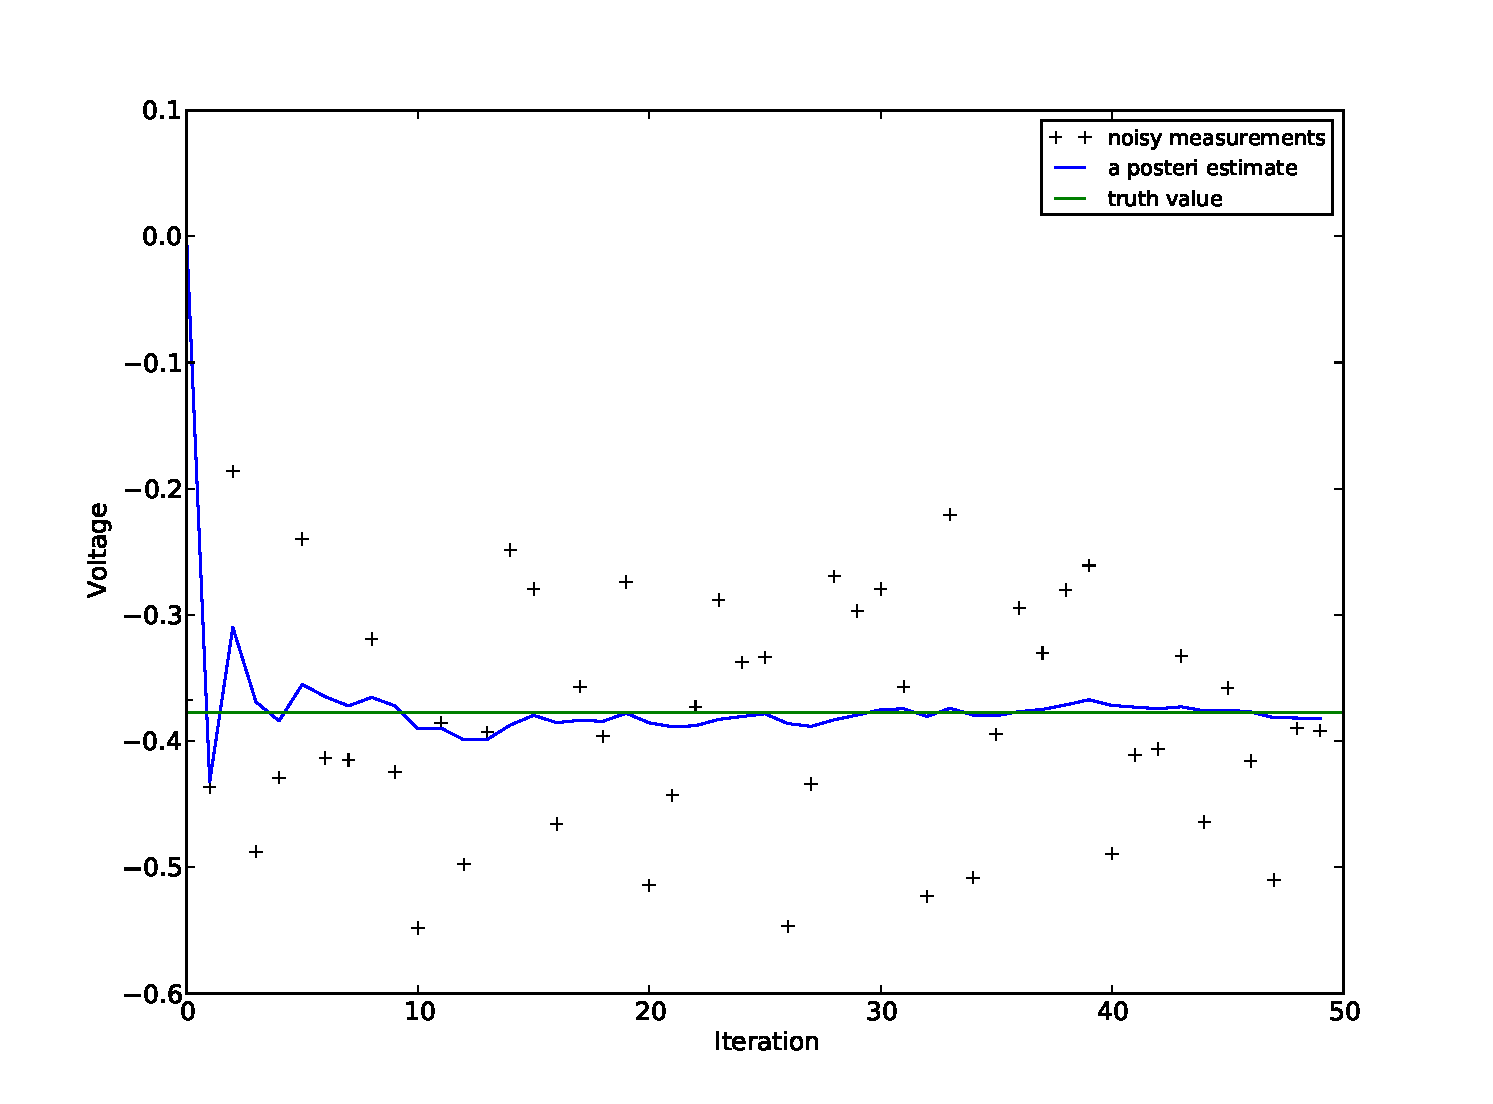
\includegraphics[width=3.0in]{../scripts/kalman.pdf}
\end{figure}

\end{frame}



\section{Conclusion}
\begin{frame}
	\frametitle{Conclusions}

\end{frame}


\begin{frame}
	\frametitle{Any Questions\ldots}

\end{frame}











\end{document}

